\section{Sonnet: All at Sea}

\begin{figure}[h]
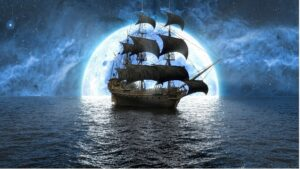
\includegraphics[width=.25\textwidth]{GhostShip-300x169.jpg}
\end{figure}

by \textbf{James Lawrence}

\begin{verse}
Night is at its nadir and the moon-scythe's light\\ Gets mocked to dizziness in the drunken sea;\\ The tomb of fish-shoals spittles up its spite,\\ And glimmering squid-hordes dream and breed in me.

Hail has hammered me in my open cot,\\ And freezing ice-floes fettered me to standstill;\\ And the sink of rivers, swelling as it rots,\\ Spreads out more wave-halls long before my land-sill.

Still I'll not despire to no mermaid's rock;\\ I plot one hundred paths to my beloved;\\ But her liquid heart sits hard behind its lock;\\ I pitch, and toss, one hundred tries rebuffèd.

The sun-brand swelters, and the salt-sick main\\ Mists up, distills this whispering refrain.
\end{verse}

\url{https://www.gornahoor.net/wp-content/uploads/2023/03/AllAtSea_Audio.m4a}



\flrightit{Posted on 2023-03-16 by Cologero}

\begin{center}* * *\end{center}

\begin{footnotesize}
\begin{sffamily}
\texttt{Mike M on 2023-03-24 at 12:04 said:}

Beautiful imagery and metaphor as well as the reading itself.

\end{sffamily}
\end{footnotesize}

